\subsubsection{Initial Test Plan}
We developed an initial plan based on our findings in the application survey.
As suggested we followed the questions discussed during the lecture.
The test plan includes evaluating and enhancing the existing artifacts, cross-checking the results found by the tools used and eventually improving the testing status.

\paragraph{Five V\&V Questions}
We started with evaluating EvaP regarding the five basic verification and validation questions:
\begin{enumerate}
	\item When do verification and validation start? When are they complete?
    
    Verification and validation started along the start of the project and will be an important part during the duration of the project. 
	\item What particular techniques should be applied during development?
    
    As EvaP is a software too big to be wholly tested by us within the scope of the seminar project, we will try to apply as many techniques as possible on a small subpart of the project. We will evaluate the techniques and make recommendations for further testing to the main developers.
	\item How can we assess the readiness of a product?
    
    Since EvaP is already in use it is certainly ready. Our testing will not influence the readiness.
	\item How can we control the quality of successive releases?
    
    Additionally to continous integrationa and automated tests, a code review before merge is already implemented in the development process to control the quality of successive releases. We hope to enable developers to gain more knowledge about the system by enhancing the available artifacts and documentation.
	\item How can the development process itself be improved?
    
    The main weakness of the development process is the sparse distribution of knowledgeand the change of developers over time. Since only students are interested in developing EvaP we do not see a possibility to improve this part of the process.
\end{enumerate}

\paragraph{Test Classifications and Approaches}
Considering the following test approaches we came to the conlusion described below:
\begin{enumerate}
    \item Validation vs. Defect Testing
    
    Since there is no requirements document or even a list of features, it is hard to implement validation testing. As we will not draw up a corresponding document, we will not apply validation testing. However, if possible, we will try to detect defects in the software by finding inputs leading to incorrect behaviour. Thus, we will apply defect testing.
    \item Development, Release, User Testing 
    
    Because of the applied continuous integration process: Development testing is already in use. Release testing and acceptance is not possible; there are no specified releases. User testing is applied in a way as most users familiar with the developer report encountered bugs directly.
    \item Unit/Component, Integration, System Testing
    
    EvaP is a web application, so there are no hardware components directly involved. While there are software dependencies, this aspect is already covered by the tool Gemnasium. For a web application it would be important to work in the most popular web browsers (desktop and mobile). Since there are no complaints known about EvaP not working in a web browser and no plans exist about developments that would use different web browser features, we will not focus on integration testing. Similar to validation testing, without a specified requirements we can not execute system testing. Instead we will focus on unit and component testing. 
\end{enumerate}
In conclusion, we will use tests to find unnoticed defects and we will apply different testing techniques on units or components of EvaP. These testing approaches align with our goals to help EvaP's developers and to learn about different testing techniques.

\paragraph{Available Artifacts}
The most thorough artifact, the GitHub wiki, offers two artifacts with potential regarding coverage-based testing:
\begin{itemize}
    \item A finite state machine describing the states of courses in the evaluation process (\ref{fig:original-states}) (\url{https://github.com/fsr-itse/EvaP/wiki/Evaluation-States})
    \item Description of a few use cases with UML use case diagrams (\url{https://github.com/fsr-itse/EvaP/wiki/Use-Cases})
\end{itemize}
\begin{figure}[h]
    \centering
    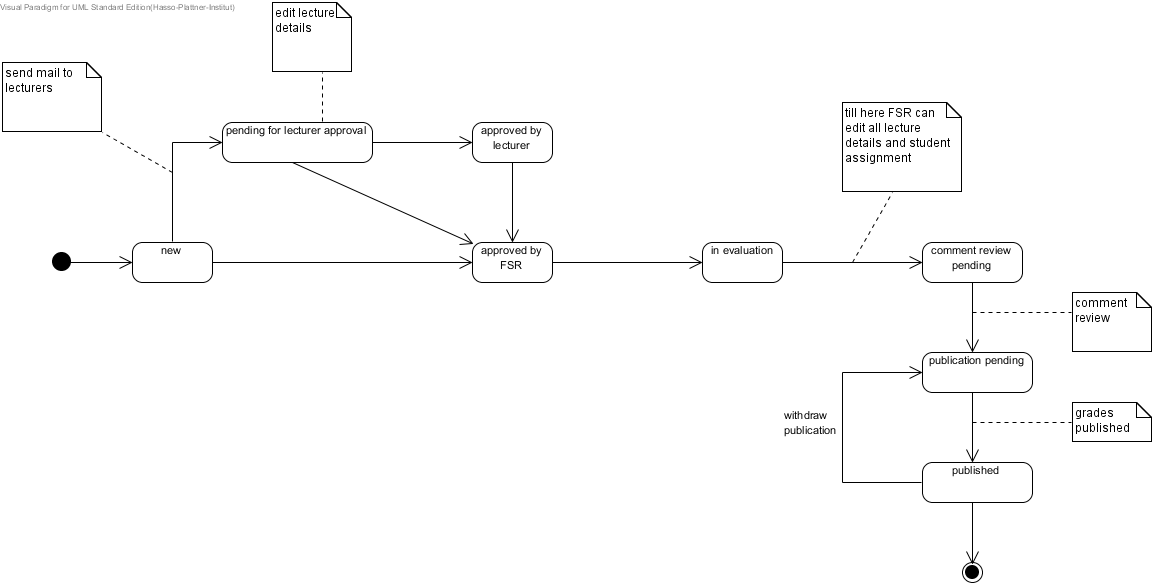
\includegraphics[width=\textwidth, keepaspectratio]{graphics/original_states_of_a_course}
    \caption{Original FSM: Possible states of a course}
    \label{fig:original-states}
\end{figure}

\paragraph{Initial Test Plan}
Based on our findings, the initial test plan is as follows:
\begin{itemize}
    \item Create a control flow graph of a function, apply coverage criteria to define test sets and implement tests
    \item Check and if necessary update the FSM of evaluation states
    \item Use or create a UML use case diagram including its elaboration to develop an activity diagram
    \item Investigate coverage found by the tool COVERALLS
\end{itemize}
